\chapter{Gap-Filling} \label{Chap4}

\section{Overview and Necessity of Gap-Filling}

FCH4 at NWFP is severely incomplete (Section 3.2.1): 56.5\% missing at Tower 4, 75.0\% at Tower 9,
and 88.5\% at Tower 2. A continuous CH\textsubscript{4} series is a precondition for every
downstream stage of this dissertation -- forecasting (Chapter~\ref{Chap5}) requires an
uninterrupted autoregressive history, and scenario projection (Chapter~\ref{Chap6}) requires a
trustworthy baseline to project from -- so gap-filling is not a preliminary data-cleaning step here
but a modelling contribution in its own right, benchmarked, uncertainty-quantified, and evaluated
against the published literature on its own terms. This chapter first replicates established
gap-filling baselines from the literature under NWFP's own conditions (Section 4.4), then improves
on them using a wider model roster, richer features, and pooling across towers (Section 4.5),
closing with the resulting champion's uncertainty quantification.

\section{Implementation Methodology}

Thirteen configurations are benchmarked in this chapter, spanning from trivial statistical floors to
tabular foundation models: a training-set mean (the trivial floor every other model must beat),
Marginal Distribution Sampling (MDS, the literature standard), Random Forest with meteorological
drivers only (RF, raw-driver baseline), MICE (multivariate imputation by chained equations),
HyperImpute (an AutoML per-column imputer), the improved, feature-enriched Random Forest (RFm, this
chapter's pooled champion, Section 4.5), LightGBM, XGBoost, TabPFN, TabICLv2 (evaluated both pooled
across towers and solo per tower), SAITS (a self-attention imputation network), and a bidirectional
LSTM (Bi-LSTM). Two further models tested during this project's development -- SVM and ANN -- appear
only in the baseline-replication comparison (Section 4.4), not in the improved-pipeline roster of
Section 4.5, since ANN's role there is specifically to replicate Kim et al.'s published comparison
and SVM underperformed consistently across every baseline-replication scenario. TabICLv2 and TabPFN
are the tabular foundation models introduced in Section~\ref{sec:tabular-modelling} -- TabICLv2 is
used here in its regression (\texttt{TabICLRegressor}) configuration; it is evaluated in both a
pooled and a solo-per-tower configuration, since its fixed 10,000-row context cap makes pooling
actively harmful for this model specifically (unlike Random Forest, which benefits from pooling,
Section 4.5.2) -- the solo configuration is this chapter's TabICLv2 headline result throughout.
Uncertainty quantification is implemented for the two strongest models: quantile-regression-forest
(QRF) intervals for RFm, and TabICLv2's native quantile-regression output, both calibrated via
conformal calibration (Section 4.5.4).

\section{Implementation Metrics and Evaluation Protocol}

The primary metric throughout this chapter is $R^2$ at hourly resolution, alongside RMSE, MAE, and
mean bias error (MBE). Every point metric reported in this chapter is the median across five
artificial-gap scenarios of increasing length -- 1 hour, 4 hours, 32 hours, 288 hours, and a mixed-
length scenario -- rather than a single fixed gap length, so that a model's score reflects its
robustness across realistic blackout durations rather than performance at one arbitrarily chosen gap
length (gap-length-specific results are reported separately in Section 4.5.3.2). All models are
evaluated under a blocked, calendar-gap cross-validation protocol with h-block buffering applied
uniformly across all three towers: contiguous calendar blocks are held out as synthetic gaps, with a
buffer window excluded from training immediately around each held-out block to prevent leakage from
temporally adjacent observations. This mirrors the evaluation paradigm used by Irvin et al., Zhu et
al., and Kim et al. (Chapter~\ref{Chap2}), and is the basis for direct comparison against their
published numbers in Section 4.4.3.

One caveat applies throughout this chapter and is stated here rather than repeated at each
comparison: $R^2$ is not computed identically across the source papers being replicated, and this
dissertation makes a deliberate, consistent choice between the two conventions in play.
Scikit-learn's residual-based $R^2$ (\texttt{sklearn.metrics.r2\_score}) is unbounded below and
penalises systematic bias as well as scatter; Zhu et al.\ instead report a correlation-squared
metric ($R^2_{OLS}$, equivalent to a squared Pearson correlation via
\texttt{scipy.stats.linregress}), bounded to $[0,1]$ and insensitive to additive bias. \textbf{This
dissertation reports $R^2_{OLS}$ as its primary gap-filling metric throughout Section 4.5} --
matching Zhu et al.'s own literature convention directly, and avoiding the interpretive burden of an
unbounded-below statistic on a benchmark whose own literature ceiling is itself reported in $R^2_{OLS}$
terms. The two conventions diverge sharply for MDS specifically (an early, uncorrected sklearn-based
comparison found a 0.30 gap against $R^2_{OLS}$ for MDS, before three implementation bugs in this
project's MDS reconstruction were corrected) but diverge only modestly for every Random Forest-,
tree-, or TabICL-based model tested. Two scoped exceptions retain the sklearn convention: Section 4.4's
replication of Irvin et al., Zhu et al., and Kim et al.'s own published baseline figures necessarily
preserves each source study's original reporting convention for a faithful comparison; and the
gap-length-robustness, daily-aggregation, and feature-ablation analyses later in Section 4.5.3 predate
this chapter's switch to $R^2_{OLS}$ and are reported in their originally-computed sklearn $R^2$,
since no $R^2_{OLS}$ recomputation exists at that finer granularity -- only Table 4.2's headline
comparison and the baseline-improvement analysis that follows it use $R^2_{OLS}$.

\section{Replication of Baseline}

\subsection{Overview of Models Used}

Three published gap-filling studies are replicated under NWFP's own data and evaluation protocol:
Irvin et al.\ (Random Forest and XGBoost against a 17-site FLUXNET-CH4 wetland benchmark), Zhu et
al.\ (Random Forest against MDS, the specific comparison this dissertation's improved pipeline is
ultimately measured against, on UK managed pasture), and Kim et al.\ (Random Forest, ANN, and MDS,
with an additional PCA-based dimensionality-reduction variant). Together these replications cover
the model families -- tree ensembles, MDS, and simple neural networks -- that dominate the existing
EC-CH4 gap-filling literature (Section~\ref{sec:tabular-modelling}).

\subsection{Overview of Features Used}

Each replication uses the feature set specified by its source paper as closely as NWFP's own data
allows: Irvin et al.'s replication uses meteorological drivers plus the co-measured EC fluxes
(latent heat, sensible heat, FCO2) their paper includes; Zhu et al.'s replication deliberately
excludes those co-measured fluxes, isolating a realistic meteorological-driver-only feature set
(labelled RFm throughout this dissertation); Kim et al.'s replication adds lagged environmental
variables and a PCA-reduced driver variant on top of the meteorological-only base.

\subsection{Results and Comparison with Cited Numbers}

\begin{table}[h]
\centering
\footnotesize
\begin{tabular}{lp{5cm}p{5cm}}
\toprule
Replication & Published result & NWFP replication ($R^2$) \\
\midrule
Irvin et al.\ (RF/XGB, 17 wetland sites) & RF $R^2$=0.79, XGB $R^2\approx$0.65--0.67 &
T4: RF 0.144, XGB 0.086; T9: RF $-$0.027, XGB $-$0.089 \\
Zhu et al.\ (RFm vs.\ MDS, UK pasture) & RF beats MDS for gaps $>$12 days; both $R^2<0.1$ &
T4: RFm $\approx-0.13$, MDS $\approx-0.20$; T9: RFm $\approx-0.10$ (best), MDS $-0.58$ for 12-day
gaps -- RF-beats-MDS finding confirmed \\
Kim et al.\ (RF/ANN/MDS/PCA) & RF best at short gaps, ANN competitive at longer gaps; PCA
degrades ML performance & T4: RF best short (+0.136), ANN best medium/long/xlong
(+0.091/+0.077/+0.057); T9: RF\_lag best short/medium (+0.152/+0.160), RF\_PCA7 best long/xlong
(+0.111/+0.056) -- PCA-degrades-ML finding \textbf{not} confirmed at NWFP \\
\bottomrule
\end{tabular}
\caption{Baseline replication results against published source figures.}
\end{table}

Two findings replicate cleanly: Random Forest beats MDS at longer gap lengths (Zhu et al.'s central
claim), and ANN becomes competitive with Random Forest at longer gap lengths (Kim et al.'s central
claim, confirmed at Tower 4). One does not replicate: Kim et al.'s finding that PCA-reduced drivers
degrade ML performance is not observed at NWFP -- PCA-reduced Random Forest instead wins at longer
gaps at Tower 9, a site-specific reversal. The magnitude gap against Irvin et al.\ (their wetland
$R^2$ of 0.79 vs.\ this dissertation's 0.144 at best) is expected rather than a replication failure:
Irvin et al.'s feature set includes co-measured EC fluxes strongly correlated with CH4 at their
sites, and NWFP's own realistic driver-only feature set (Zhu et al.'s replication, directly above)
is the fairer point of comparison for a deployable gap-filling pipeline -- the premise the improved
pipeline in Section 4.5 builds from. This early MDS/RFm replication uses Zhu et al.'s own exact
feature scope and is kept distinct from the literature-corrected MDS and raw-driver-only RF floors
reported in Section 4.5.3.1, which instead use this chapter's own final, bug-fixed implementations.

\begin{figure}[htbp]
\centering
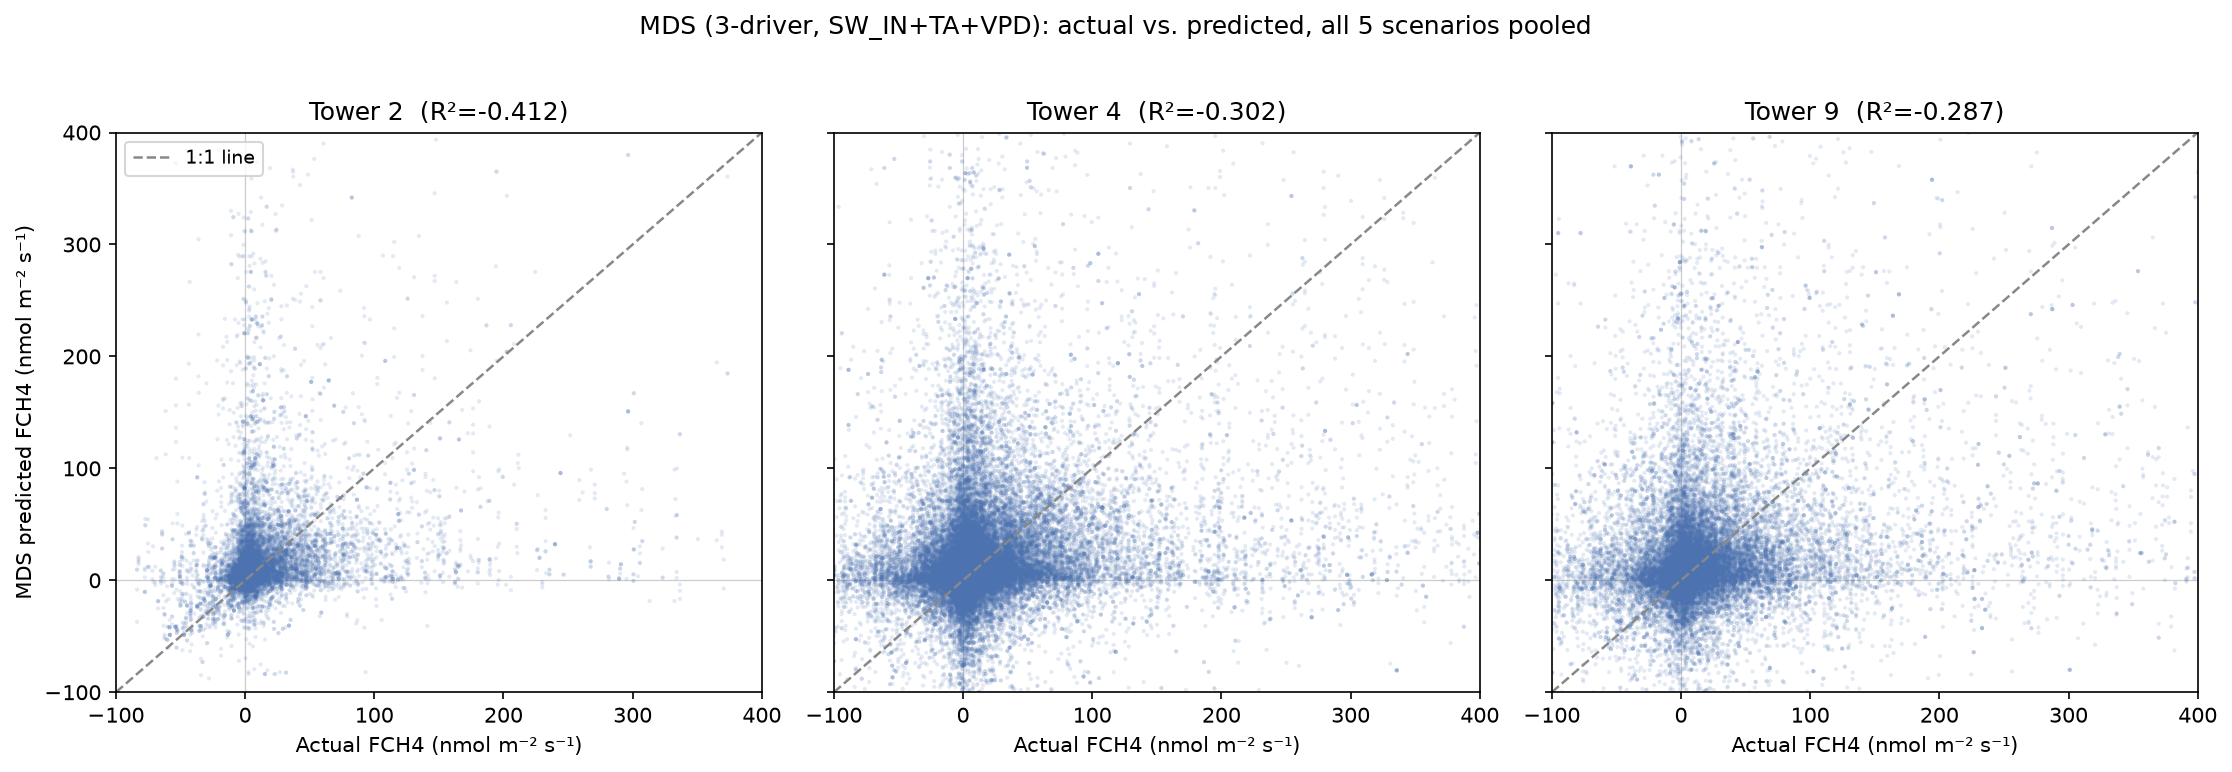
\includegraphics[width=\textwidth]{Figures/ch4_mds_scatter.png}
\caption{MDS actual-vs-predicted FCH4, all five gap-length scenarios pooled, per tower -- the
literature-standard baseline's near-zero/negative predictive skill is visible directly as scatter
around the 1:1 line rather than along it.}
\end{figure}

\FloatBarrier

\section{Improving the Baseline}

\subsection{Overview of Models Used}

Building on the RFm baseline replicated above, the improved pipeline benchmarks the full roster
introduced in Section 4.2 -- from a trivial training-set-mean floor and the literature-standard MDS,
through MICE and HyperImpute as general-purpose imputers, to RFm (this chapter's pooled champion),
LightGBM, XGBoost, TabPFN, TabICLv2 (pooled and solo), SAITS, and Bi-LSTM -- against a common
evaluation protocol (Section 4.3).

\subsection{Overview of Features Used}

\subsubsection{Pooling Approach}

RFm is fitted as a partial pool across all three towers -- a single model trained on T2+T4+T9
jointly, with tower-indicator dummy variables distinguishing catchments -- rather than three
independent per-tower models. This pooling is the single largest lever behind Tower 9's
improvement over the R-02 replication baseline (Section 4.4.3), since it lets Tower 9's shorter
individual record borrow statistical strength from Towers 2 and 4's longer records. TabICLv2 is the
deliberate exception: it is evaluated both pooled and solo, and solo per-tower fitting is
consistently the stronger configuration (Section 4.5.3.1), because its fixed context-row cap makes
pooled context actively harmful rather than helpful for this specific architecture.

\subsubsection{Additional Features}

Beyond the meteorological drivers used in the RFm baseline replication, the improved pipeline adds:
gap-filled FCO2 as a predictive feature (a proxy shown to substantially improve FCH4 prediction,
Chapter~\ref{Chap2}); livestock stocking density (LSU/ha, this project's single most important
feature, confirmed independently across gap-filling, forecasting, and scenario projection, and
returned to throughout this dissertation); pruned management-event recency features; gap-filled
meteorological drivers and GPP/Reco via the REddyProc-style pipeline described in Section 3.3.1;
and per-catchment external soil temperature. A dimensionality-reduction-informed consensus feature
selection (Section 3.2.3) identified a stable 6-variable meteorological core (soil temperature,
soil moisture, air temperature, VPD, wind speed, soil heat flux) underlying this feature set.

\subsection{Results and Comparison with Baseline}

\subsubsection{Full Model Comparison}

\begin{table}[h]
\centering
\footnotesize
\begin{tabular}{lccc}
\toprule
Model or experiment & T2 $R^2_{OLS}$ & T4 $R^2_{OLS}$ & T9 $R^2_{OLS}$ \\
\midrule
Training-set mean & 0.000 & 0.000 & 0.000 \\
MDS & 0.072 & 0.038 & 0.054 \\
RFm (meteorology only) & 0.054 & 0.042 & 0.065 \\
MICE (Bayesian ridge) & 0.104 & 0.128 & 0.110 \\
HyperImpute (AutoML) & 0.567 & 0.352 & 0.362 \\
\textbf{RFm, pooled (champion)} & 0.601 & 0.409 & \textbf{0.430} \\
LightGBM & 0.583 & 0.418 & 0.425 \\
XGBoost & 0.619 & 0.380 & 0.375 \\
TabPFN\textsuperscript{\dag} & -- & -- & -- \\
TabICLv2, pooled & 0.587 & 0.425 & 0.368 \\
SAITS & 0.562 & 0.289 & 0.304 \\
Bidirectional LSTM & 0.280 & 0.204 & 0.189 \\
\textbf{TabICLv2, solo (best raw result)} & \textbf{0.686} & \textbf{0.429} & \textbf{0.430} \\
\bottomrule
\end{tabular}
\caption{Full gap-filling model comparison: median hourly $R^2_{OLS}$ (Zhu et al.'s convention,
Section 4.3) across all five gap-length scenarios, all thirteen configurations tested.
\textsuperscript{\dag}TabPFN's $R^2_{OLS}$ was not computed -- deliberately scoped out, since its
sklearn $R^2$ (0.459/0.401/0.402) already established it as a clear loser behind every tree-based or
foundation-model result and did not warrant the additional recomputation cost.}
\end{table}

Every row of the roster is reported here, not only the final champion and its closest challenger, to
show the full build-up this dissertation's result rests on: from a trivial floor and the literature-
standard MDS baseline (both close to zero $R^2_{OLS}$, as Zhu et al.\ themselves report for this
ecosystem type), through general-purpose imputers (MICE, HyperImpute) that recover real but limited
signal, to the two models that lead this comparison. Solo-fitted TabICLv2 is this dissertation's
single best raw result, leading at Tower 2 (+0.085 over RFm) and Tower 4 (+0.020), and matching RFm
exactly at Tower 9 (0.430 for both, to three decimal places); RFm remains the stronger choice
specifically where a matching production-grade uncertainty-quantification tool has been built around
it (Section 4.5.4) -- so both are reported as this chapter's result, rather than declaring an
unqualified single winner. Pooled TabICLv2 is included alongside its solo counterpart specifically
to make this pooling effect visible: pooling costs TabICLv2 real accuracy at every tower (most
severely at Tower 9, $0.368$ vs.\ solo's $0.430$), confirming Section 4.5.2's pooling caveat directly
rather than asserting it. LightGBM and XGBoost, evaluated here as full roster members rather than
only as a challenger footnote, each edge the champion at exactly one tower under $R^2_{OLS}$
(LightGBM at Tower 4, $+0.009$; XGBoost at Tower 2, $+0.018$) but trail it at the other two; Bi-LSTM
trails across the board, and SAITS -- despite a substantial improvement over its earlier treatment in
this project's development (Section 4.5.4) -- remains behind the champion at every tower too, though
ahead of both deep-learning baselines.

One caveat applies to Tower 2's comparatively strong $R^2_{OLS}$ across every model in this section:
it reflects a discriminable livestock-on/off signal specific to Tower 2's land-use history (the
1,675-day permanent-pasture-to-arable conversion described in Section 3.2.1), not a genuinely
easier underlying prediction task -- a model at Tower 2 partly benefits from learning to
distinguish two structurally different regimes rather than from resolving finer-grained
CH4-flux variation within a single, stable regime the way Towers 4 and 9 require.

\paragraph{Improvement over the baseline.} This project's own methodological convention treats
improvement over MDS, not absolute $R^2$, as the goal (a managed-grassland ecosystem is inherently
open and noisy, so a high absolute ceiling was never expected). Table 4.2 makes that improvement
directly measurable for the first time in $R^2_{OLS}$ terms, the same units Zhu et al.\ themselves
report MDS in:

\begin{table}[h]
\centering
\begin{tabular}{lccc}
\toprule
Improvement (MDS $\rightarrow$) & T2 & T4 & T9 \\
\midrule
RFm champion & $+0.529$ & $+0.371$ & $+0.376$ \\
TabICLv2 solo (best result) & $+0.614$ & $+0.391$ & $+0.376$ \\
\bottomrule
\end{tabular}
\caption{$R^2_{OLS}$ improvement over the literature-standard MDS baseline (0.072/0.038/0.054),
this chapter's two headline results.}
\end{table}

Both the production-tooled RFm champion and the best-raw-accuracy TabICLv2 result improve on MDS by
roughly 0.37--0.61 $R^2_{OLS}$ units at every tower -- an eight-to-eleven-fold increase over MDS's
own score, not a marginal refinement. Tower 9, this project's most consistently difficult site
(Chapter~\ref{Chap7}), shows the smallest absolute gain in raw units ($+0.376$ either way) but still
represents roughly an eight-fold improvement over MDS's own $0.054$ there. This is the improvement
this dissertation is actually claiming: not a high absolute ceiling, which an open ecosystem-scale
system was never going to offer, but a large, consistent, multiple-fold gain over the published
literature standard at every tower.

\begin{figure}[htbp]
\centering
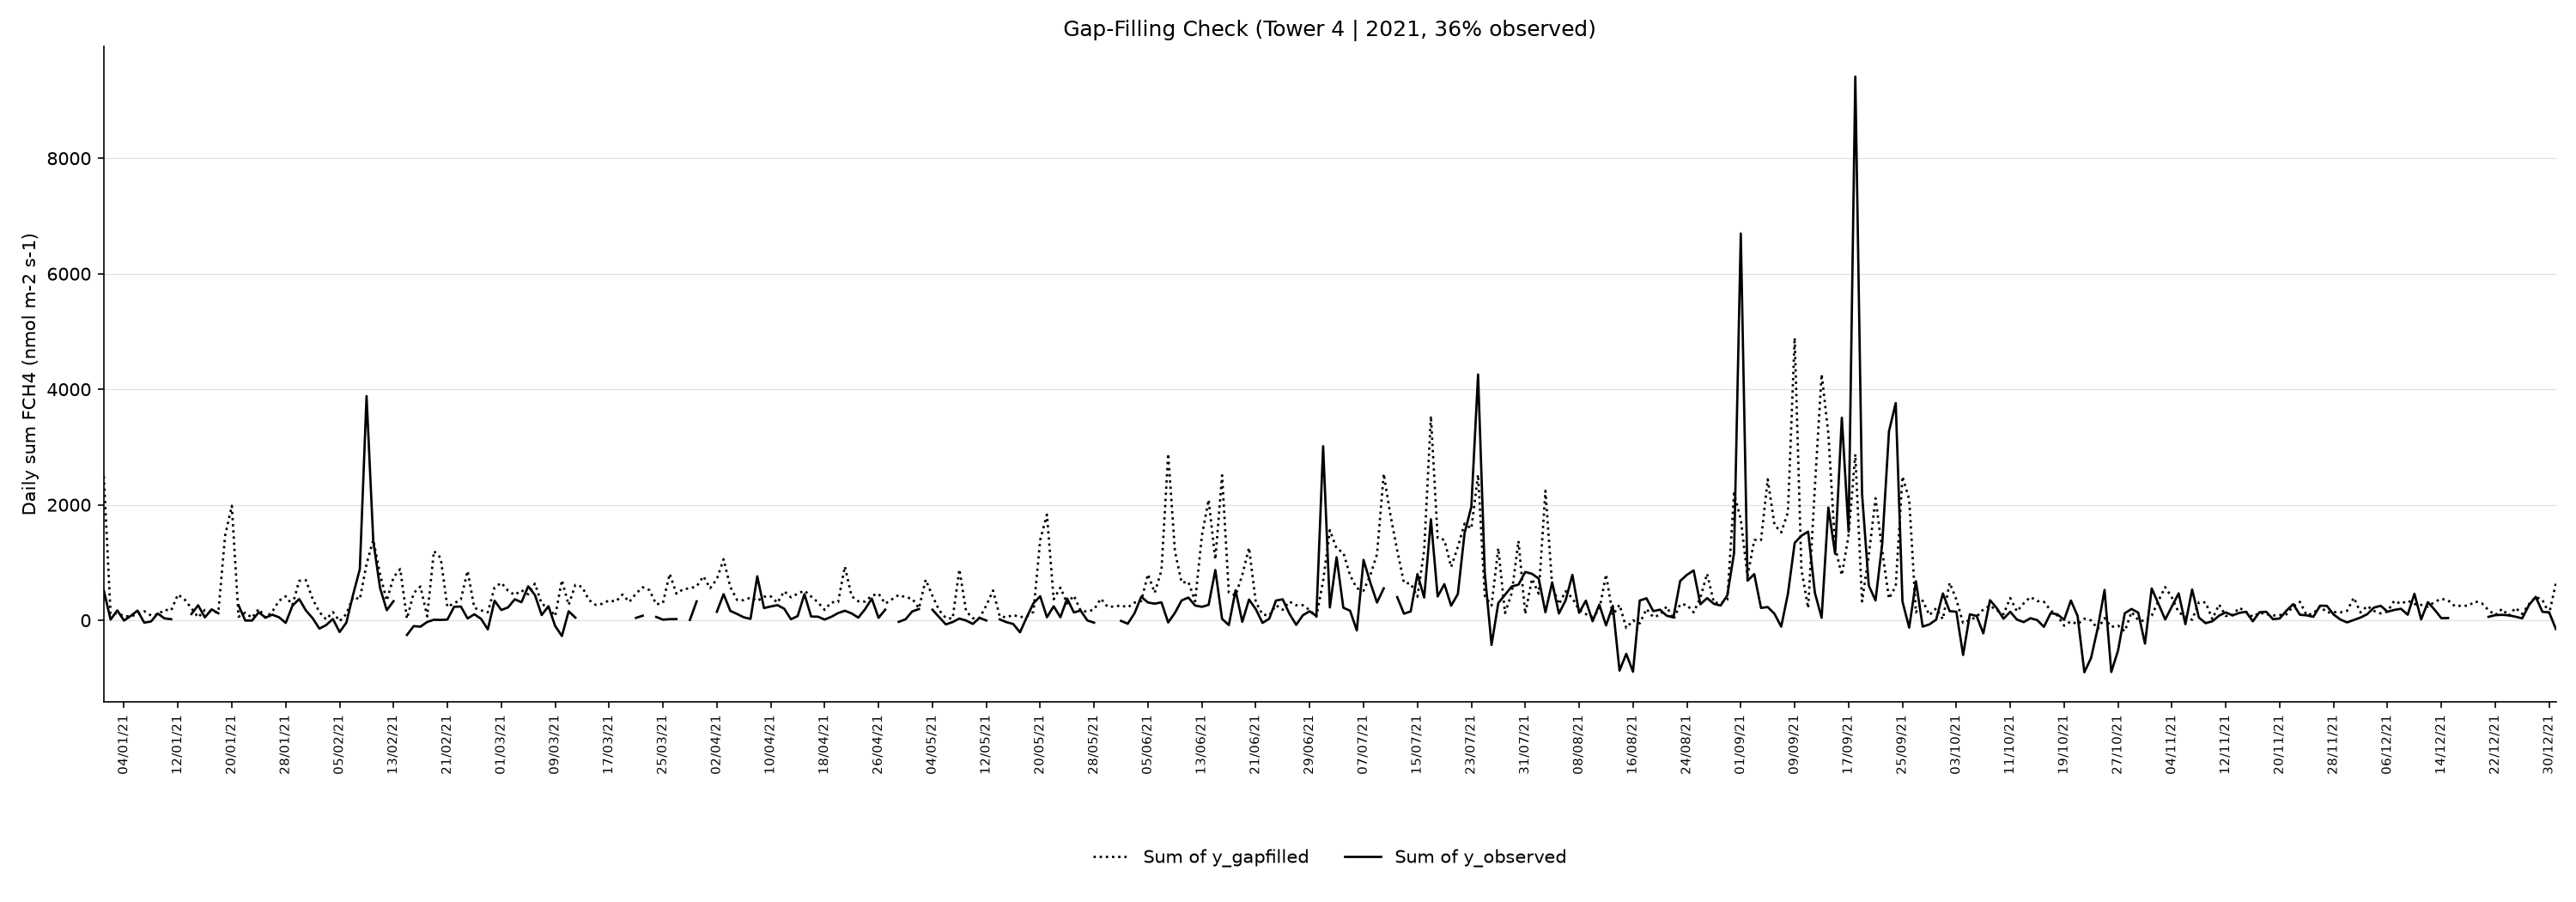
\includegraphics[width=\textwidth]{Figures/ch4_champion_chain_T4_2021.png}
\caption{Champion gap-filling check, Tower 4, 2021 (36\% observed): daily-summed real observations
against the gap-filled series produced by the improved pipeline.}
\end{figure}

\FloatBarrier

\subsubsection{Robustness to Gap Length}

\begin{table}[h]
\centering
\footnotesize
\resizebox{\textwidth}{!}{%
\begin{tabular}{lccccc}
\toprule
Model & 1 h & 4 h & 32 h & 288 h & mixed \\
\midrule
LightGBM & .522/.448/.447 & .663/.410/.406 & .646/.441/.422 & .033/.238/.177 & .470/.291/.422 \\
XGBoost & .551/.389/.445 & .671/.349/.369 & .598/.363/.383 & $-$.647/$-$.062/.060 & .143/.228/.333 \\
TabPFN & .459/.455/.443 & .704/.401/.402 & .684/.456/.543 & .092/.214/.190 & .456/.346/.350 \\
TabICLv2, pooled & .558/.461/.459 & .722/.435/.364 & .698/.423/.467 & .218/.233/.231 & .466/.332/.330 \\
SAITS & .510/.408/.378 & .219/.319/.285 & .659/.248/.338 & .055/.207/$-$.139 & .358/.293/.258 \\
Bidirectional LSTM & .423/.011/.146 & .237/.138/.150 & .546/.265/.167 & .148/.155/.072 & .189/.175/.112 \\
TabICLv2, solo & .676/.521/.514 & .727/.465/.423 & .687/.428/.459 & .057/.206/$-$.102 & .428/.291/.227 \\
\bottomrule
\end{tabular}%
}
\caption{$R^2$ by gap-length scenario, each cell T2/T4/T9.}
\end{table}

The 288-hour scenario is the clearest weakness across the entire roster: several models, including
the solo TabICLv2 champion at Tower 9, turn negative at this gap length even though their
median-across-scenarios result (Table above) is comfortably positive. The headline $R^2$ figures
reported throughout this chapter -- medians across all five scenarios -- should accordingly not be
read as evidence of equal reliability at every blackout duration; a 12-day (288-hour) blackout is
this pipeline's genuine stress case, for every model tested.

\subsubsection{Daily Aggregation and Coverage Sensitivity}

Aggregating the champion RFm's held-out hourly predictions to daily resolution raises $R^2$
noticeably at every tower (unweighted full-scope: 0.698/0.504/0.485, vs.\ the hourly 0.576/0.404/
0.426), as expected from averaging out hour-to-hour noise. This gain is sensitive to exactly how the
aggregation is defined: restricting to days with at least 50\% real hourly coverage lowers Tower 2
and Tower 4's daily $R^2$ (0.638/0.446) while raising Tower 9's (0.586); weighting each day's
contribution by its number of observed hours raises all three slightly further (0.721/0.528/0.498).
This sensitivity range is reported explicitly because a daily-resolution figure, quoted without its
aggregation rule, can be made to look more or less favourable than the underlying hourly result
supports -- this dissertation's primary reported metric throughout remains the hourly figure
(Chapter~\ref{Chap1}), with the daily figures above reported only as a sensitivity check.

\subsubsection{Feature, Pooling, and Refinement Ablations}

A wide range of feature and refinement variants were tested against the RFm/TabICLv2 champions;
almost all were neutral or negative, and are recorded here for completeness rather than presented as
adopted improvements. Replacing aggregate livestock density with species-disaggregated density
changed RF $R^2$ to 0.593/0.404/0.428 -- a small Tower 2 gain, not a general improvement. Adding
species and grazing-memory features together changed RF $R^2$ to 0.601/0.395/0.425, a similar
pattern: real at Tower 2, flat-to-negative elsewhere. A wide lag/lead feature expansion (164
features) degraded accuracy clearly (0.543/0.262/0.293 vs.\ the champion's 0.576/0.404/0.426).
Fertiliser-recency additions reduced gap-filling $R^2$ for both RF and TabICLv2. TICA-derived
components, tested as direct input features (distinct from their use as a feature-\emph{selection}
signal, Section 3.2.3), were essentially neutral; feeding a model's own prediction-interval width
back in as an input feature reduced RF's $R^2$ and severely damaged TabICLv2's, particularly at
Towers 2 and 9. TabICLv2 feature-dropping and TICA-component substitution were both flat or
negative. Native TabICLv2 hyperparameter variants stayed within $-0.025$ to $+0.019$ $R^2$ of the
default configuration -- a clean null result, nothing left on the table there. Row-cap bagging (fitting
several TabICLv2 instances on different row subsets and averaging) improved only Tower 4, from
0.428 to approximately 0.440--0.441, plateauing by five to eight bags. Confidence-gated TabICLv2
self-training (promoting high-confidence predictions into the training pool as pseudo-labels) was
neutral or harmful overall, its largest gain a marginal +0.005 $R^2$ at Tower 4.

Simple prediction-averaging across the three strongest independent models was tested as a
lower-effort alternative to further feature engineering:

\begin{table}[h]
\centering
\begin{tabular}{lccccc}
\toprule
Tower & RF & TabICLv2 & HyperImpute & RF + TabICLv2 & All three \\
\midrule
T2 & 0.576 & \textbf{0.676} & 0.509 & 0.646 & 0.621 \\
T4 & 0.404 & 0.428 & 0.336 & \textbf{0.445} & \textbf{0.445} \\
T9 & \textbf{0.426} & 0.423 & 0.354 & 0.432 & 0.417 \\
\bottomrule
\end{tabular}
\caption{Median $R^2$ under simple prediction averaging across model pairs/triples.}
\end{table}

Averaging does not produce a general replacement for solo TabICLv2 -- it loses at Tower 2, where
TabICLv2 alone is already this chapter's best individual result -- but the Tower 4 gain (0.428 to
0.445) is real and reproducible, if tower-specific rather than a general-purpose improvement.

\subsection{Uncertainty Quantification for the Champion and Best Alternative}

Both RFm and TabICLv2 have calibrated uncertainty intervals: quantile-regression-forest (QRF)
intervals for RFm, and TabICLv2's native quantile-regression output (evaluated in its pooled
configuration, matching the models this uncertainty work was originally built against).

\begin{table}[h]
\centering
\footnotesize
\begin{tabular}{llccc}
\toprule
Model & Tower & $n$ & PICP (target 0.90) & MPIW \\
\midrule
QRF (RFm) & T2 & 12,384 & 0.941 & 162.7 \\
QRF (RFm) & T4 & 48,707 & 0.919 & 197.1 \\
QRF (RFm) & T9 & 28,189 & 0.898 & 213.7 \\
TabICLv2 (quantile) & T2 & 12,384 & 0.918 & 141.7 \\
TabICLv2 (quantile) & T4 & 48,707 & 0.901 & 184.2 \\
TabICLv2 (quantile) & T9 & 28,189 & 0.893 & 220.8 \\
\bottomrule
\end{tabular}
\caption{Raw (uncalibrated) 90\% prediction interval coverage and mean width by model and tower.}
\end{table}

Raw coverage is already close to the 90\% nominal target for both models at every tower without any
calibration step. Widths correlate moderately with absolute error (Pearson $r=0.48$--$0.64$ across
the six model/tower cells, strongest for QRF at Tower 2), indicating the raw interval width carries
real, if imperfect, information about where each model is more or less likely to be wrong.

\begin{figure}[htbp]
\centering
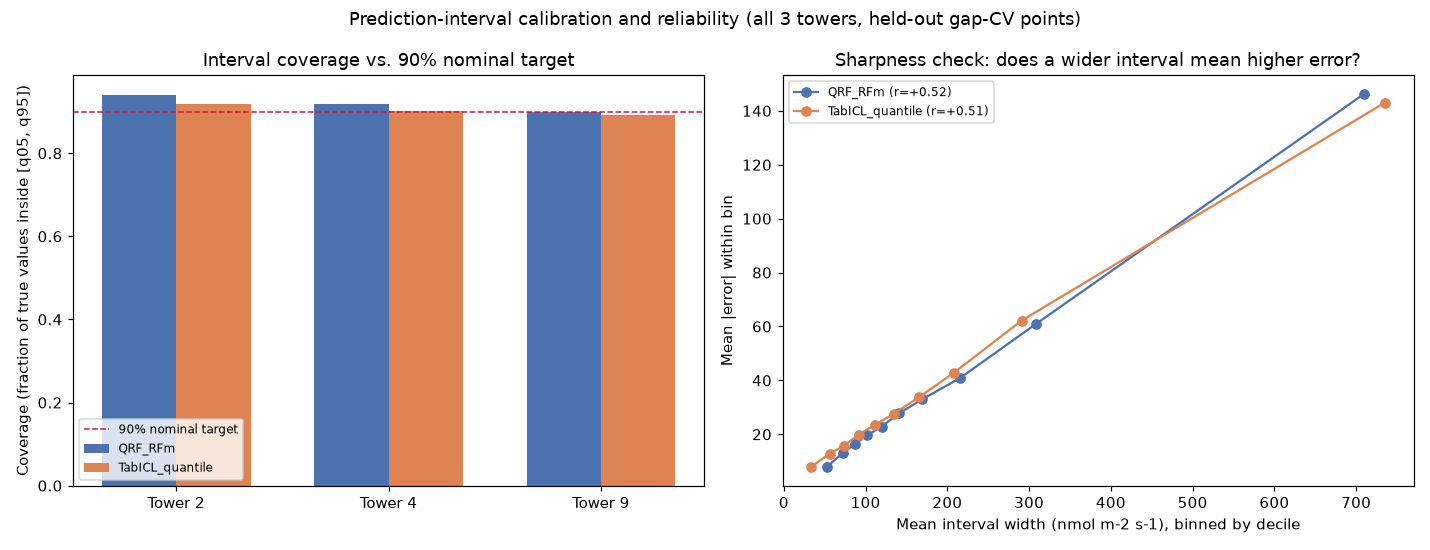
\includegraphics[width=\textwidth]{Figures/ch4_uq_calibration_reliability.png}
\caption{Prediction-interval coverage against the 90\% nominal target (left) and interval-width
sharpness against binned mean absolute error (right), QRF (RFm) vs.\ TabICLv2 quantile, all three
towers, held-out gap-CV points.}
\end{figure}

\FloatBarrier

Split-conformal calibration was applied on top of these raw intervals, moving coverage closer to
0.90 across individual tower/gap-scenario cells: calibrated QRF coverage ranged 0.876--0.912 and
calibrated TabICLv2 coverage ranged 0.888--0.910 across the cells tested, with calibration narrowing
already over-covering cells and widening under-covering ones, as intended. A separate daily-
resolution conformal calibration was also tested:

\begin{table}[h]
\centering
\begin{tabular}{lcccc}
\toprule
Tower & Calibration days & Test days & PICP & MPIW \\
\midrule
T2 & 112 & 112 & 0.866 & 104.7 \\
T4 & 430 & 430 & 0.923 & 161.5 \\
T9 & 245 & 245 & 0.861 & 124.7 \\
\bottomrule
\end{tabular}
\caption{Daily-resolution conformal calibration, RFm champion.}
\end{table}

TabICLv2 is ahead of QRF at two of three towers on the hourly comparison (Table 4.5) -- sharper
(narrower mean interval width) while sitting closer to nominal 90\% coverage, rather than QRF's more
conservative, wider-than-necessary intervals at Towers 2 and 4. This is broadly consistent with
TabICLv2 (pooled) also being a strong point-estimate model (Section 4.5.3.1), though the pooled
configuration used for this uncertainty work is not the solo configuration that is this chapter's
overall best point estimate. One limitation applies to every interval reported in this section: this
uncertainty-quantification work predates the solo-TabICLv2 point champion identified in
Section 4.5.3.1, and interval width did not reliably grow with real (as opposed to synthetic)
blackout length in the daily-resolution check above -- these intervals should accordingly not yet be
presented as fully calibrated uncertainty for the exact solo-TabICLv2 configuration this chapter
otherwise recommends as its best point estimate.
